%%%%%%%%%%%%%%%%%%%%%%
% BORROWING STRENGTH %
%%%%%%%%%%%%%%%%%%%%%%
As pointed out in \cref{sec:PEM:CombInf}, Bayesian multilevel modeling allows for ``optimal combination of information'' or ``borrowing strength''.
Here we demonstrate this inferential mechanism and investigate its underlying flow of information for the previous application example.
% QOI / NUISANCE
The Bayesian model of probabilistic inversion \cref{eq:PEM:ProbInv:Model} is considered.
However, as opposed to probabilistic inversion we declare experiment-specific elastic moduli \(\tuple{E_i}\) as the QoI whereas the hyperparameters \(\bm{\theta}_E\) are considered nuisance.
Herein we highlight the optimal inference of a single \(E_{\analyzed}\) for some \(\analyzed \in \{1,\ldots,n\}\).
\par % EXPERIMENTAL SETUP
The experimental setup is similar to the one described in \cref{sec:PEM:CaseStudies:ProbInv}.
For \(n=50\) beams, elastic moduli \(E_i\) are randomly sampled from \(\mathcal{LN}(E_i \cond \mu_E,\sigma_E)\).
Beam dimensions \(\bm{l}_i\), measurement positions \(\bm{s}_i\) and the applied loads \(F_i\) are chosen as before.
% PREDICTIONS
With \cref{eq:PEM:Beams:AlgebraicFormula} beam deflections \(\perfect{\bm{v}}_i\) are predicted.
% PSEUDO DATA
Synthetic data \(\bm{v}_i = \perfect{\bm{v}}_i + \bm{\varepsilon}_i\) are generated by perturbing the predictions \(\perfect{\bm{v}}_i\) with noise.
For this purpose noise terms \(\bm{\varepsilon}_i\) are independently sampled from Gaussian distributions \(\mathcal{N}(\bm{\varepsilon}_i \distparam \bm{0},\bm{\Sigma}_i)\).
% SYSTEMATIC EFFECTS
We choose \(\bm{\Sigma}_i = \sigma_i^2 \bm{I}_3\) with \(\sigma_i = \unit[0.1]{mm}\) for \(i \neq \analyzed\) and \(\sigma_{\analyzed} = \unit[0.1]{cm}\).
The latter describes a comparably large deviation that differs from the setup of \cref{sec:PEM:CaseStudies:ProbInv}.
This choice serves the purpose of clearly illustrating the inferential mechanism of optimal combination of information.
\par % SUMMARY
Eventually optimal combination of information reads as the following problem.
With noisy data \(\tuple{\bm{y}_i} \equiv \tuple{\bm{v}_i}\) an experiment-specific \(\bm{x}_{\analyzed} \equiv E_{\analyzed}\) has to be ideally estimated, i.e.\ taking all available sources of information into account.
The hyperparameters \(\bm{\theta}_{\bm{X}} \equiv \bm{\theta}_E\) as well as \(\tuple{\bm{x}_{\notanalyzed}} \equiv \tuple{E_{\notanalyzed}}\) are considered nuisance to that end.
Experiment-specific knowns are \(\tuple{\bm{d}_i} \equiv \tuple{(F_i,\bm{l}_i,\bm{s}_i)}\) and \(\tuple{\bm{\Sigma}_i}\).
The resultant posterior will be of the form \(\pi(\bm{x}_{\analyzed} \cond \tuple{\bm{y}_i}) \equiv \pi(E_{\analyzed} \cond \tuple{\bm{v}_i})\).
Subsequent to formulating the joint posterior \(\pi( \tuple{\bm{x}_i},\bm{\theta}_{\bm{X}} \cond \tuple{\bm{y}_i}) \equiv \pi( \tuple{E_i},\bm{\theta}_E \cond \tuple{\bm{v}_i})\), the QoI-marginals can be easily extracted.
% REMAINING SETUP
Other than that, the experimental setup of probabilistic inversion is adopted.
% DAG
Thus the experiment can be visualized by the DAG in \cref{fig:PEM:DAG:ProbInv}, too.

\subsubsection{Results: Information accumulation}
% OUTLINE
We conduct simple updating, sequential filtering and multilevel inversion for estimating \(E_{\analyzed}\), as introduced in \cref{sec:PEM:CombInf}.
%%%%%%%%%%%%%%%%%%%%%%%%%%%%%%%%%%%%%%%%%%%%%%%%%%%%%%%%%%%%%%%%%%%%%%%%%%%%%%%%%%%%%%%%%%%%%%%%%%%%%%%%%%%%%%%%%%%%%%%%%%%%%%%%%%%%%%%%%%%%%%%%%%%%%%%%%%%%%%%%%%%%%%%%%%%%%%%%%%%%%%%%%
% SIMPLE UPDATING
First of all we start with the simple Bayesian updating approach that was introduced in \cref{sec:PEM:CombInf:SimpleUpdating}.
% METHOD OF COMPOSITION
By the method of composition we draw \(K = 10^5\) samples \((E_{\analyzed}^{(1)},\ldots,E_{\analyzed}^{(K)})\) from the mixture prior \(\pi(E_{\analyzed})\) that corresponds to \cref{eq:PEM:CombInf:SimpleUpdating:Prior}.
% KDE
With this sample the mixture prior can be evaluated as the corresponding one-dimensional KDE with Gaussian kernel functions.
% POSTERIOR
The posterior \(\pi(E_{\analyzed} \cond \bm{v}_{\analyzed})\) results from conditioning on the piece of data \(\bm{v}_{\analyzed}\).
% MCMC
This univariate posterior is explored in \(N=10^5\) MCMC iterations for which the program execution time amounts to \(t=\unit[5.86]{h}\).
The final result of this simple updating approach is shown in \cref{fig:PEM:CombInf:SimpleUpdating}.
%%%%%%%%%%%%%%%%%%%%%%%%%%%%%%%%%%%%%%%%%%%%%%%%%%%%%%%%%%%%%%%%%%%%%%%%%%%%%%%%%%%%%%%%%%%%%%%%%%%%%%%%%%%%%%%%%%%%%%%%%%%%%%%%%%%%%%%%%%%%%%%%%%%%%%%%%%%%%%%%%%%%%%%%%%%%%%%%%%%%%%%%%
\par % SEQUENTIAL FILTERING
Second of all we conduct the sequential Bayesian filtering program that was proposed in \cref{sec:PEM:CombInf:SequentialFiltering}.
% MCMC % PROBABILISTIC INVERSION
In \(N=10^7\) MCMC iterations that take \(t=\unit[3.95]{h}\), probabilistic inversion for estimating \(\bm{\theta}_E\) is executed with the data \(\tuple{\bm{v}_{\notanalyzed}}\).
% METHOD OF COMPOSITION
MCMC samples from the resultant posterior \(\pi(\bm{\theta}_E \cond \tuple{\bm{v}_{\notanalyzed}})\) are used to sample the compound distribution
\(\pi(E_{\analyzed} \cond \tuple{\bm{v}_{\notanalyzed}})\) in \cref{eq:PEM:CombInf:SequentialFiltering:Prior} via the composition method.
% MIXTURE PRIOR
Subsequently a lognormal fit to these samples acts as the prior for \(E_{\analyzed}\).
% POSTERIOR
This prior and the arising posterior distribution \(\pi(E_{\analyzed} \cond \tuple{\bm{v}_{\notanalyzed}},\bm{v}_{\analyzed})\) are plotted in \cref{fig:PEM:CombInf:SequentialFiltering}.
% MCMC
In \(t = \unit[0.01]{h}\) of execution time \(N=10^5\) MCMC samples of the univariate posterior were sampled.
% INTERPRETATION
By comparison of the two posteriors in \cref{fig:PEM:CombInf:UpdatingAndFiltering}, the shrinkage of the posterior uncertainty from
\(\pi(E_{\analyzed} \cond \bm{v}_{\analyzed})\) to \(\pi(E_{\analyzed} \cond \tuple{\bm{v}_{\notanalyzed}},\bm{v}_{\analyzed})\) becomes apparent.
Both posteriors follow from conditioning on the data \(\bm{v}_{\analyzed}\), they update different priors \(\pi(E_{\analyzed})\) and \(\pi(E_{\analyzed} \cond \tuple{\bm{v}_{\notanalyzed}})\), though.
% FLOW OF INFORMATION
In the first place this proves that Bayesian priors are a valid source of information.
Moreover, this principally shows how learning about \(E_{\analyzed}\) can be indirectly supported by the evidence that \(\tuple{\bm{v}_{\notanalyzed}}\) contains with regard to \(\bm{\theta}_E\).
% FIGURES: SIMPLE UPDATING & SEQUENTIAL FILTERING
\begin{figure}[ht]
  \centering
  \begin{subfigure}[b]{0.5\textwidth}
    \centering
    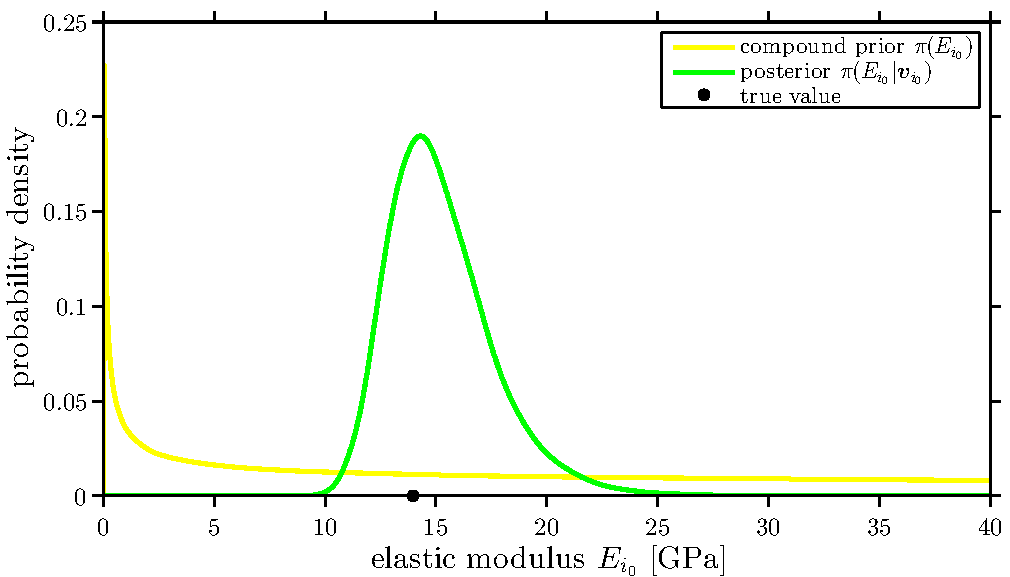
\includegraphics[height=\PEMfigHeight]{fig_PEM_CombInf1SimpleUpdating}
    \caption{Simple updating.}
    \label{fig:PEM:CombInf:SimpleUpdating}
  \end{subfigure}%
  \begin{subfigure}[b]{0.5\textwidth}
    \centering
    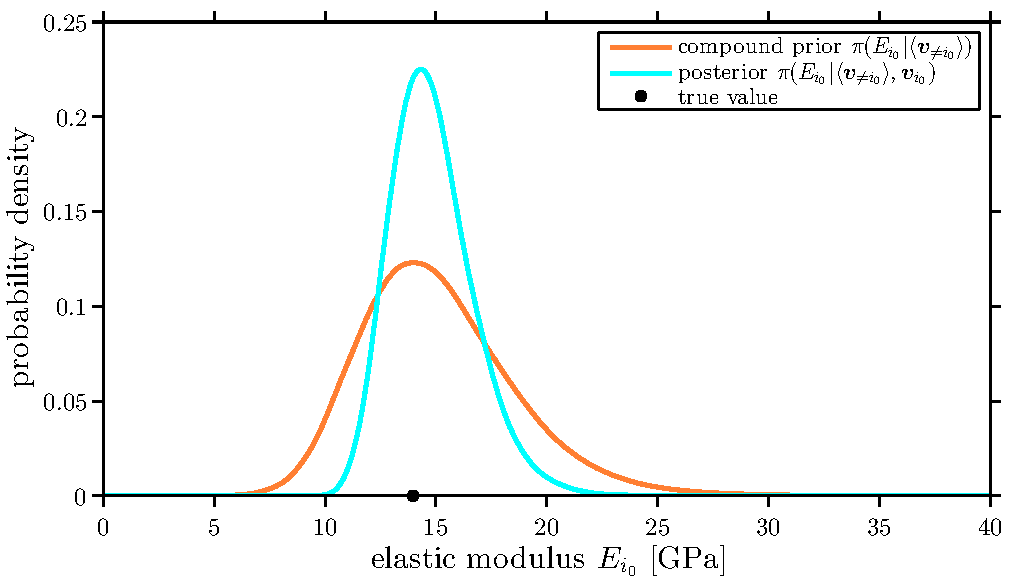
\includegraphics[height=\PEMfigHeight]{fig_PEM_CombInf1SequentialFiltering}
    \caption{Sequential filtering.}
    \label{fig:PEM:CombInf:SequentialFiltering}
  \end{subfigure}%
  \caption[Bayesian updating and filtering]{Bayesian updating and filtering.
           The mixture prior \(\pi(E_{\analyzed})\) and the posterior \(\pi(E_{\analyzed} \cond \bm{v}_{\analyzed})\) of simple updating are shown in \subref{fig:PEM:CombInf:SimpleUpdating}.
           Sequential filtering is based on the more informative mixture prior \(\pi(E_{\analyzed} \cond \tuple{\bm{v}_{\notanalyzed}})\) and the corresponding posterior
           \(\pi(E_{\analyzed} \cond \tuple{\bm{v}_{\notanalyzed}},\bm{v}_{\analyzed})\) that are given in \subref{fig:PEM:CombInf:SequentialFiltering}.
          }
  \label{fig:PEM:CombInf:UpdatingAndFiltering}
\end{figure}
%%%%%%%%%%%%%%%%%%%%%%%%%%%%%%%%%%%%%%%%%%%%%%%%%%%%%%%%%%%%%%%%%%%%%%%%%%%%%%%%%%%%%%%%%%%%%%%%%%%%%%%%%%%%%%%%%%%%%%%%%%%%%%%%%%%%%%%%%%%%%%%%%%%%%%%%%%%%%%%%%%%%%%%%%%%%%%%%%%%%%%%%%
\par % MULTILEVEL ANALYSIS
Lastly we perform Bayesian multilevel analysis as described in \cref{sec:PEM:CombInf:MultilevelAnalysis}.
% JOINT POSTERIOR
Sampling the joint posterior \(\pi(\tuple{E_i},\bm{\theta}_E \cond \tuple{\bm{v}_i})\) allows to straightforwardly extract samples
from its marginal \(\pi(E_{\analyzed} \cond \tuple{\bm{v}_{i}})\) in \cref{eq:PEM:CombInf:MultilevelAnalysis:Posterior}.
% MCMC
This is accomplished in \(t=\unit[4.57]{h}\) for \(N=10^7\) algorithm iterations.
% POSTERIORS SUMMARIES
The posterior and the previous inferential distributions relevant for \(E_{\analyzed}\) are plotted in \cref{fig:PEM:CombInf:Summary}.
In addition to that \cref{tab:PEM:CombInf:Summary} recapitulates the different approaches.
% SECOND SERIES OF RUNS
Results are also provided from a second series of runs that were independently carried out on top of the first one.
The motivation is to show that borrowing strength is a not a random but a systematic effect.
% ACCUMULATION OF INFORMATION
The accumulation of information concerning \(E_{\analyzed}\) manifests in the progressively decreasing uncertainty in the distributions.
At every stage of the estimation plan, a certain proportion of the available information has entered the analysis and has been translated into a gain of knowledge related to \(E_{\analyzed}\).
Only the multilevel posterior \(\pi(E_{\analyzed} \cond \tuple{\bm{v}_{i}})\) entirely aggregates the available information.
% FIGURES: SUMMARIES
\begin{figure}[ht]
  \centering
  \begin{subfigure}[b]{0.5\textwidth}
    \centering
    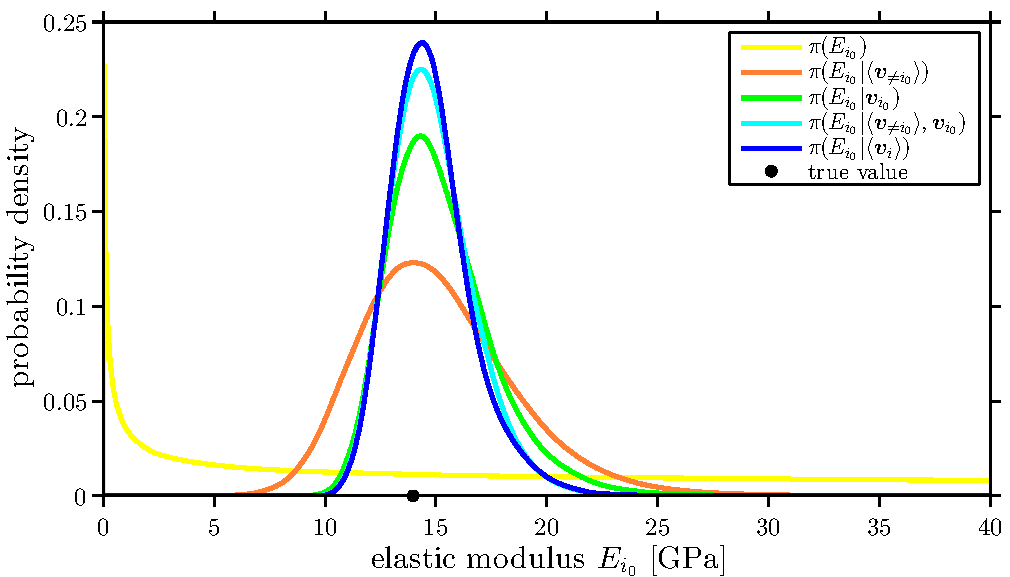
\includegraphics[height=\PEMfigHeight]{fig_PEM_CombInf1Summary}
    \caption{Summary of the \nth{1} series.}
    \label{fig:PEM:CombInf:Summary:1}
  \end{subfigure}%
  \begin{subfigure}[b]{0.5\textwidth}
    \centering
    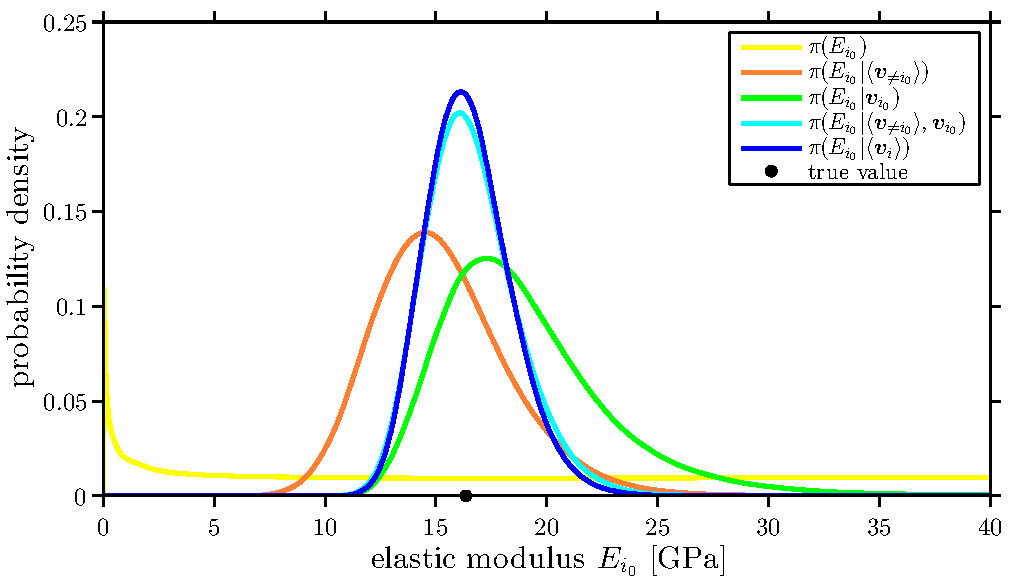
\includegraphics[height=\PEMfigHeight]{fig_PEM_CombInf2Summary}
    \caption{Summary of the \nth{2} series.}
    \label{fig:PEM:CombInf:Summary:2}
  \end{subfigure}%
  \caption[Accumulation of information]{Accumulation of information.
           In \subref{fig:PEM:CombInf:Summary:1} and \subref{fig:PEM:CombInf:Summary:2} the estimations of \(E_{\analyzed}\) are summarized for two series of runs.
           The true values are \(E_{\analyzed} = \unit[13.96]{GPa}\) and \(E_{\analyzed} = \unit[16.35]{GPa}\) in the \nth{1} and \nth{2} series, respectively.
           Uncertainties in identifying these values reflect the amount of information processed in simple updating, sequential filtering and multilevel inversion.
          }
  \label{fig:PEM:CombInf:Summary}
\end{figure}
% TABLE: OPTIMAL COMBINATION OF INFORMATION
\begin{table}[ht]
  \caption[Posterior summaries of estimating \(E_{\analyzed}\)]{Posterior summaries of estimating \(E_{\analyzed}\).}
  \label{tab:PEM:CombInf:Summary}
  \centering
  \begin{tabular}{lcccccccccc}
    \toprule
    & \phantom{} & \multicolumn{3}{c}{\nth{1} series: \(E_{\analyzed}\) \(\lbrack\unit[]{GPa}\rbrack\)} & \(\lbrack \unitless \rbrack\)
    & \phantom{} & \multicolumn{3}{c}{\nth{2} series: \(E_{\analyzed}\) \(\lbrack\unit[]{GPa}\rbrack\)} & \(\lbrack \unitless \rbrack\) \\
    \cmidrule{3-6} \cmidrule{8-11}
    && Mean & Mode & SD & CV && Mean & Mode & SD & CV \\
    \midrule
    Simple updating      && \(15.23\) & \(14.31\) & \(2.38\) & \(0.16\) && \(19.02\) & \(17.30\) & \(3.93\) & \(0.21\) \\
    Sequential filtering && \(14.82\) & \(14.32\) & \(1.83\) & \(0.12\) && \(16.58\) & \(16.07\) & \(2.03\) & \(0.12\) \\
    Multilevel inversion && \(14.75\) & \(14.37\) & \(1.79\) & \(0.12\) && \(16.47\) & \(16.12\) & \(1.85\) & \(0.11\) \\
    \bottomrule
  \end{tabular}
\end{table}
\par % UNCERTAIN LOADS
The assumption of well-known loads \(F_i\) may be overly optimistic in experimental practice.
As done in \cref{sec:PEM:CaseStudies:AddPres} one could attach an additional prescribed uncertainty to those model inputs.
In doing so we expect similar results accompanied by a weakening of borrowing strength.
% UNCERTAIN LOADS
Furthermore we expect an indirect form of borrowing strength also to occur for the inputs of a prescribed uncertainty type.
Actually the prescribed uncertainty model does not permit for learning about a specific \(F_{\analyzed}\) by borrowing strength directly from \(\tuple{\bm{v}_{\notanalyzed}}\).
However, by optimally estimating \(E_{\analyzed}\) also learning \(F_{\analyzed}\) would be indirectly strengthened.